% !TeX spellcheck = it_IT
\newpage
\section{Algebra relazionale}
L'\textbf{algebra relazionale} è l'insieme degli operatori su relazioni che danno come risultato relazioni. Viene usato come rappresentazione interna delle interrogazioni e non come linguaggio di interrogazione dei DBMS.\\
Il \textbf{calcolo relazionale} è invece il linguaggio dichiarativo di tipo logico dal quale è stato derivato SQL.

\subsection{Notazione}
\paragraph{Nomi di relazioni} $R, S, \ldots$
\paragraph{Nomi di attributi} $A, B, C, A_1, A_2, \ldots$
\paragraph{Insiemi di attributi} $X, Y, X_1, \ldots$
\paragraph{Unione di insiemi di attributi} $X \cup Y = XY$
\paragraph{Relazione con ennuple} Date le ennuple $t_1, t_2, \ldots, t_n$ la relazione è denotata con $\{t_1, t_2, \ldots, t_n\}$
\paragraph{Relazione vuota} $\{\}$
\paragraph{Valore attributo} Data la ennupla $t_k$, il suo valore $A_i$ è denotato da $t_k.A_i$
\paragraph{Ennupla specifica ad attributi} Se $X$ è sottoinsieme degli attributi di $t$, $t.X$ o $t[X]$ allora denota l’ennupla ottenuta da $t$ considerando solo gli attributi in $X$
\paragraph{Ambiguità} Se $R$ ed $S$ hanno lo stesso attributo $A_j$, in caso di ambiguità, $R.A_j$ denota l’attributo $A_j$ della relazione $R$ ed $S.A_j$ denota l’attributo $A_j$ della relazione $S$.

\newpage
\subsection{Operatori primitivi}
\subsubsection{Ridenominazione}
Viene utilizzato per cambiare il nome di una relazione e di conseguenza anche il suo \textbf{tipo}.
\begin{equation}
	\rho_{A \leftarrow B}(R)
\end{equation}
\begin{equation}
	T' = \rho_{A \leftarrow A'}(T)
\end{equation}
\begin{table}[!h]
	\centering
	\begin{tabular}{|c|c|c|}
		\hline
		\textbf{Id} & \textbf{Nome} & \textbf{Età} \\
		\hline
		7274 & Rossi & 42 \\
		\hline
		7432 & Neri & 54 \\
		\hline
		9824 & Verdi & 45 \\
		\hline
	\end{tabular}
	\hspace{10pt} $\longrightarrow$ \hspace{10pt}
	\begin{tabular}{|c|c|c|}
		\hline
		\textbf{Matricola} & \textbf{Nome} & \textbf{Età} \\
		\hline
		7274 & Rossi & 42 \\
		\hline
		7432 & Neri & 54 \\
		\hline
		9824 & Verdi & 45 \\
		\hline
	\end{tabular}
	\caption{Laureati}
\end{table}

\subsubsection{Unione}
Restituisce la relazione ottenuta facendo l’unione delle ennuple di $R$ con quelle di $S$ dove $R$ e $S$ sono relazioni dello stesso tipo.

\begin{equation}
	R \cup S
\end{equation}

\begin{table}[!h]
	\centering
	\begin{tabular}{|c|c|c|}
		\hline
		\textbf{\underline{A}} & \textbf{\underline{B}} & \textbf{\underline{C}} \\
		\hline
		a1 & b1 & c1 \\
		\hline
		a1 & b1 & c2 \\
		\hline
		a2 & b1 & c1 \\
		\hline
		a3 & b1 & c1 \\
		\hline
	\end{tabular}
	\hspace{10pt} $\cup$ \hspace{10pt}
	\begin{tabular}{|c|c|c|}
		\hline
		\textbf{\underline{A}} & \textbf{\underline{B}} & \textbf{\underline{C}} \\
		\hline
		a1 & b1 & c1 \\
		\hline
		a1 & b2 & c2 \\
		\hline
	\end{tabular}
	\hspace{10pt} $\longrightarrow$ \hspace{10pt}
	\begin{tabular}{|c|c|c|}
		\hline
		\textbf{A} & \textbf{B} & \textbf{C} \\
		\hline
		a1 & b1 & c1 \\
		\hline
		a1 & b1 & c2 \\
		\hline
		a1 & b2 & c2 \\
		\hline
		a2 & b1 & c1 \\
		\hline
		a3 & b1 & c1 \\
		\hline
	\end{tabular}
\end{table}
\subsubsection{Differenza}
Restituisce la relazione contenente le ennuple di $R$ non presenti in $S$.

\begin{equation}
	R-S
\end{equation}

\begin{table}[!h]
	\centering
	\begin{tabular}{|c|c|c|}
		\hline
		\textbf{\underline{A}} & \textbf{\underline{B}} & \textbf{\underline{C}} \\
		\hline
		a1 & b1 & c1 \\
		\hline
		a1 & b1 & c2 \\
		\hline
		a2 & b1 & c1 \\
		\hline
		a3 & b1 & c1 \\
		\hline
	\end{tabular}
	\hspace{10pt} $-$ \hspace{10pt}
	\begin{tabular}{|c|c|c|}
		\hline
		\textbf{\underline{A}} & \textbf{\underline{B}} & \textbf{\underline{C}} \\
		\hline
		a1 & b1 & c1 \\
		\hline
		a1 & b2 & c2 \\
		\hline
	\end{tabular}
	\hspace{10pt} $\longrightarrow$ \hspace{10pt}
	\begin{tabular}{|c|c|c|}
		\hline
		\textbf{A} & \textbf{B} & \textbf{C} \\
		\hline
		a1 & b1 & c2 \\
		\hline
		a2 & b1 & c1 \\
		\hline
		a3 & b1 & c1 \\
		\hline
	\end{tabular}
\end{table}

\newpage
\subsubsection{Proiezione}
Restituisce una relazione i cui elementi sono la copia delle ennuple di $R$ proiettate (ristrette) sugli attributi $A_1,\ldots, A_n$. Eventuali ennuple che dopo la proiezione sono uguali appaiono solo una volta.
\begin{equation}
	\pi_{A_1, \ldots, A_n} (R)
\end{equation}
Data la tabella usata negli esempi precedenti, la proiezione è:
\begin{table}[!h]
	\centering
	$\pi_A(R)=$ \hspace{10pt}
	\begin{tabular}{|c|}
		\hline
		\textbf{A} \\ 
		\hline
		a1 \\
		\hline
		a2 \\
		\hline
		a3\\
		\hline
	\end{tabular}
\end{table}
\paragraph{Cardinalità}
Una proiezione conterrà al più tante ennuple quanto l'operando:
\begin{itemize}
	\item  Se $X$ è una \textbf{superchiave} di $R$, allora $\pi_X(R)$ contiene esattamente tante ennuple quante $R$
	\item \textbf{Altrimenti} potrebbero esistere valori ripetuti su quegli attributi, che quindi vengono rappresentati una sola volta
\end{itemize}

\subsubsection{Restrizione o selezione}
Restituisce una relazione dello stesso tipo (schema) di $R$ i cui elementi sono la copia delle ennuple di $R$ (un sottoinsieme) che soddisfano la condizione $\phi$ definita come:
\begin{itemize}
	\item $A_i \phi A_j$ con $A_i$ e $A_j$ attributi di $R$ e $\theta$ un operatore di confronto $\{<, >, =, \neq, \leq, \geq \}$
	\item $A_i \theta c$ oppure $c \theta A_i$, con $\theta$ operatore di confronto e $c$ costante nel dominio di $A_i$
	\item Se $\phi$ e $\psi$ sono formule, allora lo sono anche $\phi \land \psi$, $\phi \lor \psi$ e $\neg \psi$
\end{itemize}
\begin{equation}
	\sigma_\phi(R)
\end{equation}
Data la tabella usata negli esempi precedenti abbiamo
\begin{table}[!h]
	\centering
	$\sigma_{A=a_1}(R)=$ \hspace{10pt}
	\begin{tabular}{|c|c|c|}
		\hline
		\textbf{A} & \textbf{B} & \textbf{C}\\ 
		\hline
		a1 & b1 & c1\\
		\hline
		a1 & b1 & c2\\
		\hline
	\end{tabular}
\end{table}

\begin{observation}[Valori nulli]
	La presenza di valori \textbf{nulli} negli attributi usati per la restrizione portano all'assenza di \textbf{atomicità} nell'operazione.
	\begin{equation*}
		\sigma_{\text{Età}>30}(\text{Persone}) \cup \sigma_{\text{Età}\leq30}(\text{Persone}) \neq \text{Persone}
	\end{equation*}
	Per mantenerla è quindi necessario utilizzare i costrutti \textit{IS NULL} e \textit{IS NOT NULL}:
	\begin{equation*}
		\sigma_{\text{Età}>30}(\text{Persone}) \cup \sigma_{\text{Età}\leq30}(\text{Persone}) \cup \sigma_{\text{Età IS NULL}}(\text{Persone}) = \text{Persone}
	\end{equation*}
\end{observation}

\newpage
\subsubsection{Prodotto}
Con $R$ e $S$ relazioni con attributi distinti, il loro prodotto è una relazione con elementi ottenuti concatenando ogni ennupla di $R$ con ogni ennupla di $S$. La relazione risultante ha grado uguale alla somma dei gradi degli operandi e cardinalità uguale al prodotto delle cardinalità degli operandi.
\begin{equation}
	R \times S
\end{equation}
\begin{table}[!h]
	\centering
	\begin{tabular}{|c|c|c|}
		\hline
		\textbf{\underline{A}} & \textbf{\underline{B}} & \textbf{\underline{C}} \\
		\hline
		a1 & b1 & c1 \\
		\hline
		a1 & b1 & c2 \\
		\hline
		a2 & b1 & c1 \\
		\hline
		a3 & b1 & c1 \\
		\hline
	\end{tabular}
	\hspace{10pt} $\times$ \hspace{10pt}
	\begin{tabular}{|c|c|}
		\hline
		\textbf{A'} & \textbf{D} \\
		\hline
		a1 & d1 \\
		\hline
		a2 & d2 \\
		\hline
	\end{tabular}
	\hspace{10pt} $\longrightarrow$ \hspace{10pt}
	\begin{tabular}{|c|c|c|c|c|}
		\hline
		\textbf{A} & \textbf{B} & \textbf{C} & \textbf{A'} & \textbf{D} \\
		\hline
		a1 & b1 & c1 & a1 & d1 \\
		\hline
		a1 & b1 & c1 & a2& d2 \\
		\hline
		a1 & b1 & c2 & a1 & d1 \\
		\hline
		a1 & b1 & c2 & a2 & d2 \\
		\hline
		a2& b1 & c1 & a1 & d1 \\
		\hline
		a2 & b1 & c1 & a2 & d2 \\
		\hline
		a3 & b1 & c1 & a1 & d1 \\
		\hline
		a3 & b1 & c1 & a2 & d2 \\
		\hline		
	\end{tabular}
\end{table}

\begin{observation}
	Il prodotto di due relazioni è un’operazione che di solito non si usa da sola. Pertanto per concatenare ennuple in associazione, si restringe sempre il prodotto alle ennuple con valore uguale della chiave esterna e chiave primaria. Per questa si introduce un operatore derivato, chiamato \textbf{giunzione}, per riferirsi alla combinazione di queste due operazioni.
\end{observation}

\subsection{Operatori derivati}
\subsubsection{Intersezione}
Restituisce la relazione ottenuta facendo l’intersezione delle ennuple di $R$ con quelle di $S$ dove $R$ e $S$ sono relazioni dello stesso tipo.

\begin{equation}
	R \cap S = R - (R-S)
\end{equation}

\begin{table}[!h]
	\centering
	\begin{tabular}{|c|c|c|}
		\hline
		\textbf{\underline{A}} & \textbf{\underline{B}} & \textbf{\underline{C}} \\
		\hline
		a1 & b1 & c1 \\
		\hline
		a1 & b1 & c2 \\
		\hline
		a2 & b1 & c1 \\
		\hline
		a3 & b1 & c1 \\
		\hline
	\end{tabular}
	\hspace{10pt} $\cap$ \hspace{10pt}
	\begin{tabular}{|c|c|c|}
		\hline
		\textbf{\underline{A}} & \textbf{\underline{B}} & \textbf{\underline{C}} \\
		\hline
		a1 & b1 & c1 \\
		\hline
		a1 & b2 & c2 \\
		\hline
	\end{tabular}
	\hspace{10pt} $\longrightarrow$ \hspace{10pt}
	\begin{tabular}{|c|c|c|}
		\hline
		\textbf{A} & \textbf{B} & \textbf{C} \\
		\hline
		a1 & b1 & c1 \\
		\hline
	\end{tabular}
\end{table}

\subsubsection{Inner Join}
Restituisce la relazione contenente le ennuple del prodotto cartesiano di $R \times S$ con valori uguali per gli attributi $A_i$ e $A_j$ dove $R$ e $S$ sono relazioni di tipo diverso (con attributi distinti) tra i quali c’è $A_i$ in $R$ e $A_j$ in $S$.
\begin{equation}
	R \Join_{A_i = A_j}S = \sigma_{A_i=A_j}(R \times S)
\end{equation}
Date le tabelle usate come esempio nel prodotto ($R$ e $T'$), abbiamo
\begin{table}[!h]
	\centering
	$R \Join_{A=A'}T' =$ \hspace{10pt}
	\begin{tabular}{|c|c|c|c|c|}
		\hline
		A & B & C & A' & D \\
		\hline
		a1 & b1 & c1 & a1 & d1 \\
		\hline
		a1 & b1 & c2& a1 & d1 \\
		\hline
		a2 & b1 & c1 & a2 & d2 \\
		\hline
	\end{tabular}
\end{table}

\subsubsection{Theta Join}
È il caso più generale della \textit{Inner Join}: qui la condizione $\theta$ è una congiunzione di termini logici di confronto ($>$, $<$, $=$, $\ldots$).
\begin{equation}
	R \Join_\sigma S
\end{equation}

\subsubsection{Natural Join}
È una abbreviazione dell’\textit{Inner Join} applicata a relazioni in cui l’associazione fra le ennuple è
descritta con la chiave esterna e la chiave primaria costituite da attributi uguali. Restituisce la relazione contenente le ennuple di $R \times S$ con gli attributi di uguali nomi in $R$ ed $S$ definiti sugli stessi domini. 
\begin{equation}
	R \Join S = R \Join_{A=A}S = \sigma_{A=A}(R \times S)
\end{equation}

\begin{table}[!h]
	\centering
	\begin{tabular}{|c|c|c|}
		\hline
		\textbf{\underline{A}} & \textbf{\underline{B}} & \textbf{\underline{C}} \\
		\hline
		a1 & b1 & c1 \\
		\hline
		a1 & b1 & c2 \\
		\hline
		a2 & b1 & c1 \\
		\hline
		a3 & b1 & c1 \\
		\hline
	\end{tabular}
	\hspace{10pt} $\Join$ \hspace{10pt}
	\begin{tabular}{|c|c|}
		\hline
		\textbf{\underline{A}} & \textbf{D} \\
		\hline
		a1 & d1 \\
		\hline
		a2 & d2 \\
		\hline
	\end{tabular}
	\hspace{10pt} $\longrightarrow$ \hspace{10pt}
	\begin{tabular}{|c|c|c|c|}
		\hline
		\textbf{A} & \textbf{B} & \textbf{C} & \textbf{D} \\
		\hline
		a1 & b1 & c1 & d1\\
		\hline
		a1 & b1 & c2 & d1 \\
		\hline
		a2 & b1 & c1 & d2 \\
		\hline
	\end{tabular}
\end{table}

\begin{note}
	Si noti che:
	\begin{itemize}
		\item Se $R$ ed $S$ non hanno attributi comuni allora $R \Join S = R \times S$
		\item Se $R$ ed $S$ hanno lo stesso schema allora $R \Join S = R \cap S$
	\end{itemize}
\end{note}

\paragraph{Cardinalità} Date le relazioni $R_1(A,B)$ e $R_2(B, C)$:
\begin{itemize}
	\item Il numero di ennuple della loro join è:
	\begin{equation*}
		0 \leq \lvert R_1 \Join R_2 \rvert \leq \lvert R_1 \rvert \times \lvert R_2 \rvert
	\end{equation*}
	\item Se il loro join è \textbf{completo} allora contiene un numero di ennuple almeno uguale al massimo tra $\lvert R_1 \rvert$ e $\lvert R_2 \rvert$
	\item Se il join coinvolge una \textbf{chiave} $B$ di $R_2$ allora:
	\begin{equation*}
		0 \leq \lvert R_1 \Join R_2 \rvert \leq \lvert R_1 \rvert 
	\end{equation*}
	\item Se il join coinvolge una \textbf{chiave} $B$ di $R_2$ e un \textbf{vincolo di integrità referenziale} tra gli attributi di $R_1$ e la chiave di $R_2$ allora:
	\begin{equation*}
		\lvert R_1 \Join R_2 \rvert = \lvert R_1 \rvert
	\end{equation*}
\end{itemize}

\begin{observation}[Natural Join e Proiezione]
	Osserviamo che valgono due cose:
	\begin{itemize}
		\item Dati $R_1(X_1)$ e $R_2(X_2)$ vale
		\begin{equation}
			\pi_{X_1}(R_1 \Join R_2) \subseteq R_1
		\end{equation}
		\item Dati $R(X)$ con $X = X_1 \cup X_2$ vale
		\begin{equation}
			R \subseteq (\pi_{X_1}(R)) \Join (\pi_{X_2}(R))
		\end{equation}
	\end{itemize}
\end{observation}

\newpage
\subsubsection{Semi Join}
Restituisce le ennuple di $R$ che partecipano alla giunzione naturale di $R$ ed $S$ con $A_1, A_2, \ldots, A_m$ attributi di $R$.
\begin{equation}
	R S = \pi_{A_1, A_2, \ldots, A_m}(R \Join S)
\end{equation}
Considerando l'esempio precedente abbiamo
\begin{table}[!h]
	\centering
	$R T =$\hspace{10pt}
	\begin{tabular}{|c|c|c|}
		\hline
		\textbf{A} & \textbf{B} & \textbf{C} \\
		\hline
		a1 & b1 & c1 \\
		\hline
		a1 & b1 & c2 \\
		\hline
		a2 & b1 & c1 \\
		\hline
	\end{tabular}
\end{table}

\subsubsection{External Join}
Il join esterno estende con valori nulli le ennuple che verrebbero tagliate fuori da un join interno. Ne esistono tre versioni:
\begin{itemize}
	\item \textbf{Left}: mantiene tutte le ennuple del primo operando, estendendole con valori nulli se necessario
	\begin{equation}
		R \overset{\leftarrow}{\Join}S
	\end{equation}
	\item \textbf{Right}: come left ma con il secondo operando
	\begin{equation}
		R \overset{\rightarrow}{\Join} S
	\end{equation}
	\item \textbf{Full}: come left ma con entrambi gli operandi
	\begin{equation}
		R \overset{\leftrightarrow}{\Join} S
	\end{equation}
\end{itemize}

\subsubsection{Self Join}
Questa operazione è utilizzata quando va fatta una join di una tabella con se stessa. Spesso è importante fare anche delle ridenominazioni.

\begin{example}[Nonno nipote]
	Data la relazione
	\begin{table}[!h]
		\centering
		\begin{tabular}{|c|c|}
			\hline
			\textbf{Genitore} & \textbf{Figlio} \\
			\hline
			Luca & Anna \\
			\hline
			Maria & Anna \\
			\hline
			Giorgio & Luca\\
			\hline
			Silvia & Maria \\
			\hline
			Enzo & Maria\\
			\hline
		\end{tabular}
	\end{table}
	effettuiamo le seguenti operazioni
	\begin{equation*}
		\rho_{\text{Genitore}, \text{Figlio} \leftarrow \text{Nonno}, \text{Genitore}}(\text{Genitore}) \Join \rho_{\text{Figlio} \leftarrow \text{Nipote}}(\text{Genitore})
	\end{equation*}
	\begin{table}[!h]
		\centering
		\begin{tabular}{|c|c|}
			\hline
			\textbf{Nonno} & \textbf{Genitore} \\
			\hline
			Luca & Anna \\
			\hline
			Maria & Anna \\
			\hline
			Giorgio & Luca\\
			\hline
			Silvia & Maria \\
			\hline
			Enzo & Maria\\
			\hline
		\end{tabular}
		\hspace{10pt} $\Join$ \hspace{10pt}
		\begin{tabular}{|c|c|}
			\hline
			\textbf{Genitore} & \textbf{Nipote} \\
			\hline
			Luca & Anna \\
			\hline
			Maria & Anna \\
			\hline
			Giorgio & Luca\\
			\hline
			Silvia & Maria \\
			\hline
			Enzo & Maria\\
			\hline
		\end{tabular}
		\hspace{10pt} $=$ \hspace{10pt}
		\begin{tabular}{|c|c|c|}
			\hline
			\textbf{Nonno} & \textbf{Genitore} & \textbf{Nipote} \\
			\hline
			Giorgio & Luca & Anna \\
			\hline
			Silvia & Maria & Anna \\
			\hline
			Enzo & Maria & Anna \\
			\hline
		\end{tabular}
	\end{table}
\end{example}

\subsection{Proprietà algebriche degli operatori}
Un'espressione algebrica può essere rappresentata come un \textbf{albero}:
\[
\begin{aligned}
	& \pi_{\text{Nome}, \text{Matricola}} (\\
	& \qquad \pi_{\text{Nome}, \text{Matricola}}(\sigma_{\text{Provincia} = \text{'PI'}}(\text{Studenti}))\\
	& \qquad \Join_{\text{Matricola} = \text{Candidato}} \\
	& \qquad \pi_{\text{Candidato}} (\sigma_{\text{Voto}=25}(\text{Esami})) \\
	&)
\end{aligned}
\qquad
\raisebox{-20mm}{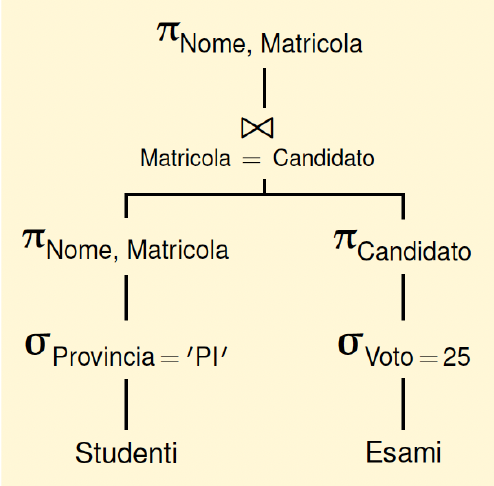
\includegraphics[scale=0.25]{albero.png}}
\]
Un’espressione dell’algebra relazionale può essere trasformata in un’altra equivalente sfruttando alcune proprietà degli operatori. Questo aiuta a ridurre il costo di esecuzione. Le proprietà più utili sono quelle che permettono di anticipare la \textbf{restrizione} e la \textbf{proiezione}:
\begin{itemize}
	\item \textbf{Raggruppamento} di \textbf{restrizioni}
	\begin{equation*}
		\sigma_{C_1}(\sigma_{C_2}(R)) \equiv \sigma_{C_1 \land C_2}(R)
	\end{equation*}
	\item \textbf{Raggruppamento} di \textbf{proiezioni}
	\begin{equation*}
		\sigma_{C_1 \land C_2}(R \times S) \equiv\sigma_{C_1}(R) \times \sigma_{C_2}(S)
	\end{equation*}
	\item \textbf{Commutatività} della \textbf{restrizione}, \textbf{proiezione}, \textbf{prodotto}, \textbf{giunzione} e degli \textbf{operatori insiemistici}
	\begin{equation*}
		(R \times S) \equiv(S \times R)
	\end{equation*}
	\item \textbf{Anticipazione} della \textbf{restrizione} rispetto al prodotto e alla giunzione e rispetto agli operatori insiemistici
	\item \textbf{Anticipazione} della \textbf{proiezione} rispetto al prodotto e alla giunzione e rispetto agli operatori insiemistici
	\item Eliminazioni di proiezioni superflue
	\begin{equation*}
		\pi_{A}(\pi_{A,B}(R)) \equiv \pi_{A}(R)
	\end{equation*}
\end{itemize}

\begin{observation}[Non distributività della proiezione rispetto alla differenza]
	In generale vale che
	\begin{equation}
		\pi_A(R_1 - R_2) \neq \pi_A (R_1)-\pi_A(R_2)
	\end{equation}
\end{observation}

\newpage
\subsection{Quantificatori}
Esistono tre tipi di quantificatori:
\begin{itemize}
	\item \textbf{Esistenziale}: e.g. tutti gli studenti che hanno preso \textit{almeno} un voto maggiore di $28$
	\item \textbf{Differenza}: e.g. tutti gli studenti che NON hanno mai preso un voto maggiore di $28$
	\item \textbf{Universale}: e.g tutti gli studenti che hanno preso SOLO voti maggiori di $28$
\end{itemize}
\begin{figure}[!h]
	\centering
	\begin{minipage}{.3\textwidth}
		\centering
		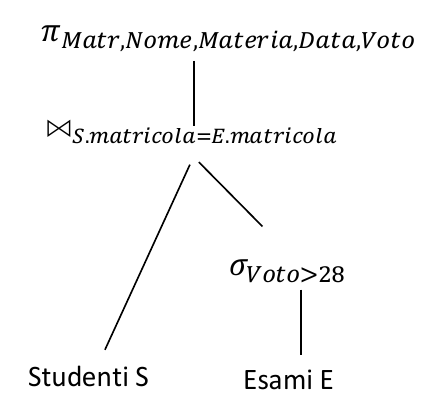
\includegraphics[scale=0.25]{esistenziale.png}
		\captionof{figure}{Esistenziale}
	\end{minipage}
	\begin{minipage}{.3\textwidth}
		\centering
		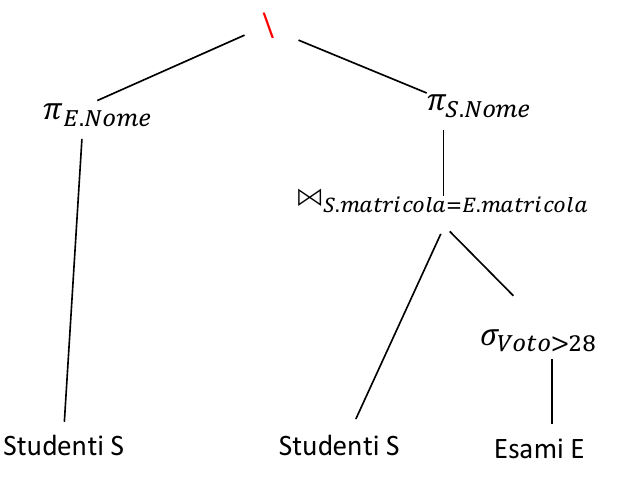
\includegraphics[scale=0.2]{differenza.png}
		\captionof{figure}{Differenza}
	\end{minipage}
	\begin{minipage}{.3\textwidth}
	\centering
	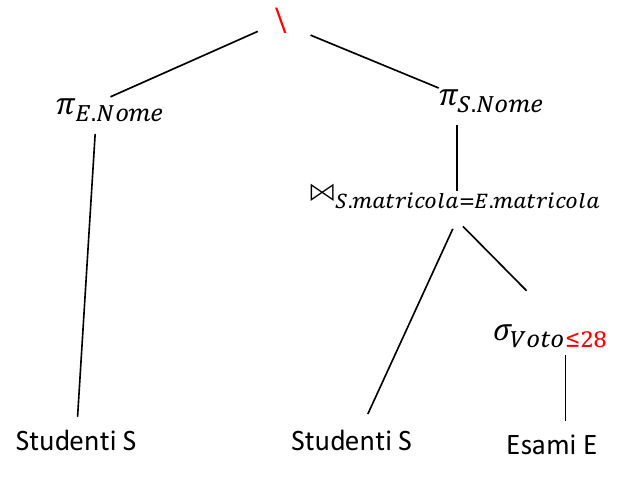
\includegraphics[scale=0.2]{universale.png}
	\captionof{figure}{Universale}
	\end{minipage}
\end{figure}

\subsection{Operatori non insiemistici}
\subsubsection{Group By}
Data una relazione $R$, i suoi attributi $A_i$ e le espressioni che usano funzioni di aggregazione $f_i$ (min, max, count, sum, $\ldots$), definiamo il raggruppamento come una relazione calcolata:
\begin{enumerate}
	\item  Partizionando le ennuple di $R$ mettendo nello stesso gruppo tutte le ennuple con valori uguali degli $A_i$
	\item Si calcolano le espressioni $f_i$ per ogni gruppo
	\item Per ogni gruppo si restituisce una sola ennupla con come attributi i valori degli $A_i$ e delle espressioni $f_i$
\end{enumerate}	
\begin{equation}
	\prescript{}{\{A_i\}\gamma\{f_i\}}{(R)}
\end{equation}
Il raggruppamento gode dell'\textbf{anticipazione} rispetto alla proiezione:
\begin{equation}
	\sigma_C(\prescript{}{X\gamma F}{(R)}) \equiv \prescript{}{X\gamma F}{(\sigma_C(R))}
\end{equation}
\begin{example}
	Vogliamo ottenere per ogni candidato il numero degli esami, il voto minimo, massimo e medio:
	\begin{equation*}
		\prescript{}{\{\text{Candidato}\} \gamma \{\text{count}(*), \min(\text{Voto}), \max(\text{Voto}), \text{avg}(\text{Voto})\}}{(\text{Esami})}
	\end{equation*}
	\begin{table}[!h]
		\centering
		\begin{tabular}{|c|c|c|c|}
			\hline
			\textbf{Materia} & \textbf{Candidato} & \textbf{Voto} & \textbf{Docente} \\
			\hline
			DA & $1$ & $20$ & $10$ \\
			\hline
			LFC & $2$ & $30$ & $20$ \\
			\hline
			MTI & $1$ & $30$ & $30$ \\
			\hline
			LP & $2$ & $20$ & $40$ \\
			\hline
		\end{tabular}\\
		\vspace{10pt} $\downarrow$ \vspace{10pt}\\	
		\begin{tabular}{|c|c|c|c|c|}
			\hline
			\textbf{Candidato} & \textbf{Count(*)} & \textbf{min(Voto)} & \textbf{max(Voto)} & \textbf{avg(Voto)} \\
			\hline
			1 & 2 & 20 & 24 & 22 \\
			\hline
			2 & 2 & 20 & 30 & 25 \\
			\hline
		\end{tabular}
	\end{table}
\end{example}
\subsubsection{Proiezione generalizzata}
Estende la proiezione con la possibilità di usare costanti o espressioni aritmetiche nella lista degli attributi. Permette anche di aggiungere \textbf{etichette} alle espressioni tramite l'operatore \textbf{AS}:
\begin{equation}
	\pi_{e_1\text{ AS } \text{ide}_1, e_2\text{ AS } \text{ide}_2, \ldots}(R)
\end{equation}
Dove $e_1, e_2, \ldots$ sono espressioni aritmetiche ottenute a partire da costanti e $\text{ide}_1, \text{ide}_2, \ldots$ sono etichette distinte.
\subsubsection{Proiezione multi-insiemistica}
Funziona come la proiezione ma senza eliminazione dei duplicati. Restituisce dei multi-insiemi e quindi si possono utilizzare solo come radice di un albero logico.
\begin{equation}
	\pi^b_{\{A_i\}}(R)
\end{equation}
\subsubsection{Ordinamento}
Ordina tutte le ennuple di $R$ in ordine crescente o decrescente rispetto agli attributi $A_i$.
\begin{equation}
	\tau_{\{A_i\}}(R)
\end{equation}

\subsection{Calcolo relazionale}
Il calcolo relazionale è un linguaggio che permette di definire il risultato di un’interrogazione (\textbf{query}) come l’insieme di quelle ennuple che soddisfano una certa condizione $\phi$.\\

L’algebra dà la possibilità di scrivere espressioni in cui gli operatori sono applicati al risultato di altri operatori (espressioni annidate). Il calcolo ha una \textbf{struttura piatta} ma permette di esprimere condizioni più \textbf{complesse}.\\
Un linguaggio che si colloca a metà tra i due stili si può ottenere:
\begin{enumerate}
	\item Aggiungendo al calcolo la possibilità di annidare il costruttore di insiemi
	\item Aggiungendo all’algebra la possibilità di avere nell’operatore di restrizione	condizioni che fanno uso anche di quantificatori e di predicati di appartenenza.
\end{enumerate}
Il risultato è un linguaggio che ha sia la capacità di esprimere interrogazioni in modo annidato che la possibilità di esprimere condizioni logiche complesse, come accade nel linguaggio SQL.

\begin{example}
	L’insieme delle matricole degli Studenti che hanno superato qualcuno degli esami elencati nella relazione Materie, si può definire come
	\begin{align*}
		& \{t.\text{Matricola} \vert t \in \text{Studenti}, \exists m \in \text{Materie}. \exists e \in \text{ProveEsami}.\\
		& e.\text{Candidato}=t.\text{Matricola} \land e.\text{Materia} = m.\text{Materia}\}
	\end{align*}
	che equivale a
	\begin{equation*}
		\pi_{\text{Matricola}}(\text{Studenti} \underset{\text{Matricola} = \text{Candidato}}{\Join}(\text{ProveEsami} \Join \text{Materie}))
	\end{equation*}
\end{example}